% 2010 年辽宁卷文科第 19 题：棱柱 ABC-A1B1C1，点 D 在 A1C1 上。
% 来源 PDF：普通高考/2010/2010辽宁文.pdf，SHA-256 b402a859318cb9854e9b8257ea128e84f1d52e834556dd80625e883f88dea1fd。
% 原页：第 2 页（A3 三栏）第 1 栏上部，书页码 614。
% 重绘依据：照原页投影像——A1、C1 在最高处同一水平线上，D 在 A1C1 上（图中居于中点），
%   B1 落在直观图内部；A 在左下、C 在右且与 A 近乎等高，B 在最下方。
%   实线：棱柱可见棱 A1C1、A1A、C1C、A1B1、B1C1、B1B、AB、BC，以及两个辅助平面与截面
%   的边 A1B、BC1、AB1、B1C、B1D；虚线：被遮挡的 AC 与截面边 DC。
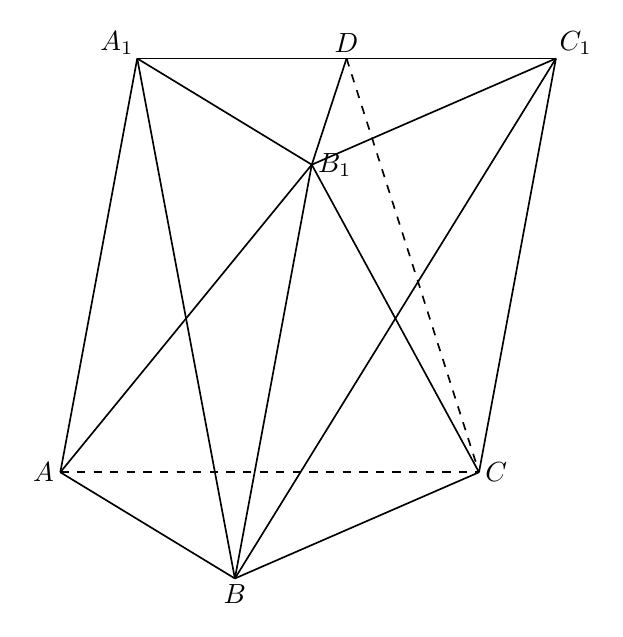
\begin{tikzpicture}[scale=1.55, semithick, line join=round]
  \coordinate (A)  at (0,0);
  \coordinate (B)  at (1.43,-0.87);
  \coordinate (C)  at (3.43,0);
  \coordinate (A1) at (0.63,3.39);
  \coordinate (B1) at (2.06,2.52);
  \coordinate (C1) at (4.06,3.39);
  \coordinate (D)  at (2.345,3.39);

  % 可见棱
  \draw (A1) -- (C1);
  \draw (A1) -- (A);
  \draw (C1) -- (C);
  \draw (A1) -- (B1);
  \draw (B1) -- (C1);
  \draw (B1) -- (B);
  \draw (A) -- (B);
  \draw (B) -- (C);

  % 平面 A1BC1 与平面 AB1C 的边（实线）
  \draw (A1) -- (B);
  \draw (C1) -- (B);
  \draw (A) -- (B1);
  \draw (B1) -- (C);

  % 截面 B1CD（B1D、B1C 已画；DC 被遮挡）
  \draw (B1) -- (D);

  % 被遮挡的棱与线段（虚线）
  \draw[dashed] (A) -- (C);
  \draw[dashed] (D) -- (C);

  % 顶点标注
  \node[above left, inner sep=1pt] at (A1) {$A_1$};
  \node[above, inner sep=2pt] at (D) {$D$};
  \node[above right, inner sep=1pt] at (C1) {$C_1$};
  \node[right=1pt, inner sep=1pt] at (B1) {$B_1$};
  \node[left, inner sep=2pt] at (A) {$A$};
  \node[below, inner sep=2pt] at (B) {$B$};
  \node[right, inner sep=2pt] at (C) {$C$};
\end{tikzpicture}
